\documentclass[tikz,border=8pt]{standalone}
\usepackage[T1]{fontenc}\usepackage{lmodern}\usepackage{pgfplots}\pgfplotsset{compat=1.18}
\begin{document}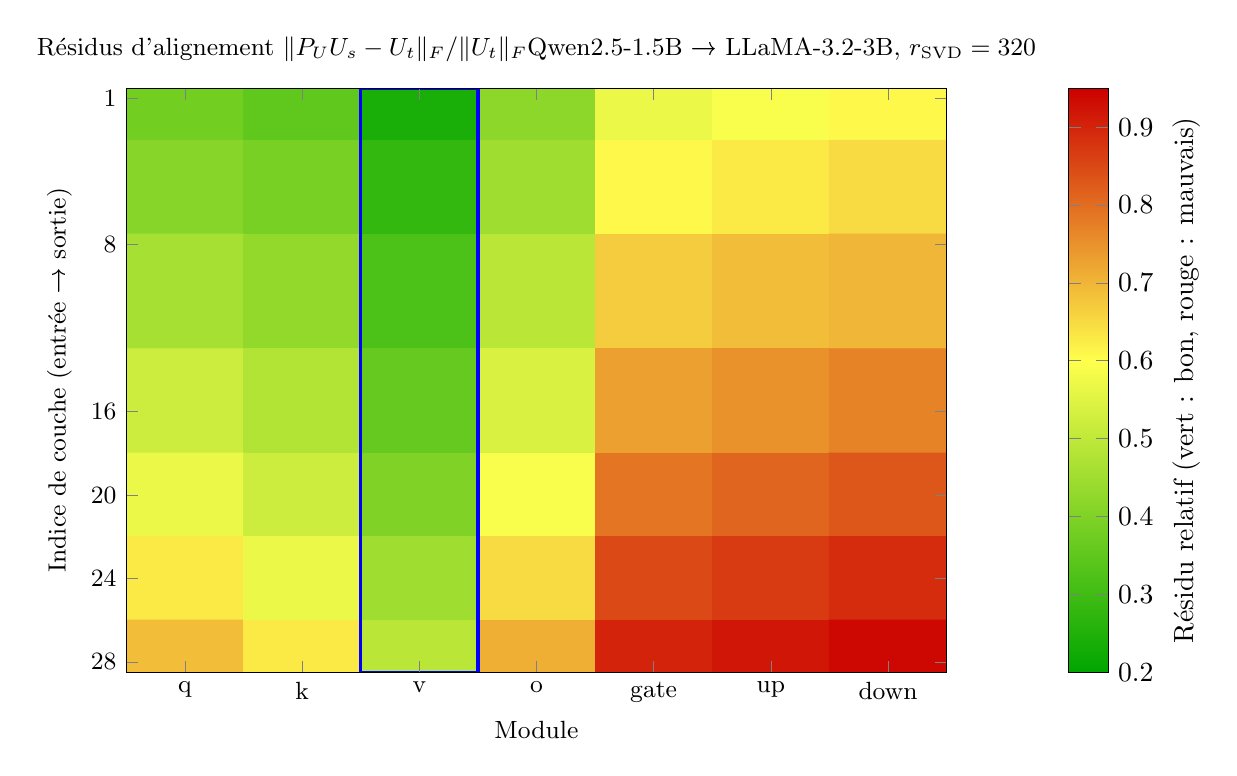
\begin{tikzpicture}
\begin{axis}[width=12cm,height=9cm,font=\small,title={Résidus d'alignement $\|P_UU_s-U_t\|_F/\|U_t\|_F$\\Qwen2.5-1.5B → LLaMA-3.2-3B, $r_{\mathrm{SVD}}=320$},xlabel={Module},ylabel={Indice de couche (entrée → sortie)},xmin=.5,xmax=7.5,ymin=.5,ymax=28.5,xtick={1,...,7},xticklabels={q,k,v,o,gate,up,down},ytick={1,8,16,20,24,28},y dir=reverse,point meta min=.2,point meta max=.95,colormap={resid}{color(0cm)=(green!65!black);color(0.4cm)=(yellow!70);color(0.75cm)=(red!80!black)},colorbar,colorbar style={ylabel={Résidu relatif (vert : bon, rouge : mauvais)}},axis on top]
% Values are illustrative: source graphic specifies trends, article reports only typical ranges.
\addplot[matrix plot*,mesh/cols=7,point meta=explicit] coordinates {
(1,1)[.38](2,1)[.35](3,1)[.24](4,1)[.42](5,1)[.57](6,1)[.59](7,1)[.61]
(1,5)[.41](2,5)[.39](3,5)[.28](4,5)[.45](5,5)[.61](6,5)[.63](7,5)[.65]
(1,10)[.46](2,10)[.43](3,10)[.32](4,10)[.49](5,10)[.67](6,10)[.69](7,10)[.70]
(1,16)[.52](2,16)[.48](3,16)[.36](4,16)[.54](5,16)[.73](6,16)[.75](7,16)[.77]
(1,20)[.57](2,20)[.52](3,20)[.40](4,20)[.59](5,20)[.79](6,20)[.81](7,20)[.83]
(1,24)[.63](2,24)[.57](3,24)[.45](4,24)[.65](5,24)[.85](6,24)[.87](7,24)[.89]
(1,28)[.69](2,28)[.63](3,28)[.49](4,28)[.71](5,28)[.90](6,28)[.92](7,28)[.94]
};
\draw[blue,very thick] (axis cs:2.5,.5) rectangle (axis cs:3.5,28.5);
\end{axis}\end{tikzpicture}\end{document}
